%!TEX root = main.tex

\section{Applications}
\label{sec:applications}

Our IVM framework supports a wide range of application scenarios. 
In this section, we highlight four seemingly disparate scenarios: 
learning regression models, building Chow-Liu trees, 
computing conjunctive query results in either listing or factorized representation, 
and multiplying a sequence (chain) of matrices.
{\em All these scenarios are treated uniformly using delta view trees
over the space of the view keys. They differ however in the rings used to define the view payloads.}

\nop{
% In this section, we highlight two scenarios, matrix chain computation and gradient computation for learning linear regression models over joins,
% % \nop{conjunctive query evaluation and safe plans in probabilistic databases.} 
% in which the payloads have sizes independent of the input relation sizes. We also highlight two distinct scenarios, where the payloads may have arbitrarily large sizes: they can be entire relations under either listing or factorized representations. 
}

\nop{
In this section, we present payload rings that can be used for static and dynamic query evaluation in our framework. We first discuss some standard sum-product rings of numbers and then introduce novel rings for learning regression models in machine learning, evaluating queries on probabilistic databases, and factorizing query computation. The modularity of our framework allows us to treat all these different rings in a uniform way. 

%%%%%%%%%%%%%%%%%%%%%%%%%%

\subsection{Sum-product Rings of Numbers}

Our framework captures a wide range of problems that can be expressed as sum/count aggregates over numerical values. Some examples include conjunctive query evaluation, graphical model inference, constraint satisfaction, counting subgraphs of a massive graph, and matrix multiplication. 
% 
Our framework stores aggregate values as payloads rather than as separate columns like in SQL. This data model simplifies incremental processing as changing aggregate values of tuples amounts to changing their payloads rather than deleting tuples with old aggregate values and inserting tuples with new aggregate values.

When computing {\tt COUNT} aggregates in our framework, the payload is from $\mathbb{Z}$ and the lift function of every bound variable in a view tree is $\LIFTFN(x) = 1$. Figure~\ref{fig:example_intro_viewtree} shows a view tree and the contents of each view for our example query and the given database instance.

For computing {\tt SUM} aggregates over a product of functions of one variable, the payload is from a ring of numbers (e.g., $\mathbb{Z}$, $\mathbb{Q}$, etc.) and the lift function of a bound variable $X$ is the function with which $X$ appears in the {\tt SUM} expression; otherwise, $\LIFTFN(x) = 1$ (see Example~\ref{ex:sql_sum_aggregate}). For \texttt{AVG} aggregates, the payload consists of a pair of count and sum aggregates, and $+$ and $*$ are pairwise addition and multiplication. 
}


%%%%%%%%%%%%%%%%%%%%%%%%%%%%
\subsection{Covariance Matrix and Linear Regression}
%\subsection{Gradient Computation for Learning Linear Regression Models over Joins}
\label{sec:application-lr}

We next introduce a ring for the computation of the covariance matrix for training linear regression models.

\paragraph{\textbf{Linear Regression.}}
Consider a training dataset that consists of $k$ samples with $(X_i)_{i\in[m-1]}$ features and a label $X_m$ arranged into a design matrix ${\bf M}$ of size $k \times m$; in our setting, this design matrix is the result of a join query. The goal of linear regression is to learn the parameters $\Th = \TR{[\theta_1 \ldots \theta_m]}$ of a linear function\footnote{We consider wlog: $\theta_1$ is the bias parameter and then $X_1=1$ for all tuples in the input data; $\theta_m$ remains fixed to $-1$ and corresponds to the label/response $X_m$ in the data.} $f(X_1,\ldots,X_{m-1}) = \sum_{i\in[m]}\theta_iX_i$ best satisfying ${\bf M} \Th \approx {\bf 0}_{k\times 1}$, where ${\bf 0}_{k\times 1}$ is the zero matrix of size $k \times 1$.

We can solve this optimization problem using batch gradient descent. This method iteratively updates the model parameters in the direction of the gradient to decrease the squared error loss and eventually converge to the optimal value. Each convergence step iterates over the entire training dataset to update the parameters, $\Th := \Th - \alpha\TR{\bf M}{\bf M}\Th$, where $\alpha$ is an adjustable step size. The complexity of each step is $\bigO{mk}$. The {\em covariance matrix}  $\TR{\bf M}{\bf M}$ quantifies the degree of correlation for each pair of features (or feature and label) in the data. Its computation can be done once for all convergence steps~\cite{SOC:SIGMOD:2016}. This is crucial for performance in case $m \ll k$ as each iteration step now avoids processing the entire training dataset and takes time $\bigO{m^2}$. 

\nop{
Computing the covariance matrix $\TR{\X}\X$, which quantifies the degree of correlation for each pair of features, can be expensive. When $\X$ is the result of an equi-join query $Q$ over database $\db$, computing $\TR{\X}\X$ taking a flat join result as input would take $\bigO{m^2 \cdot |\db|^{\rho^{*}(Q)}}$ time. But computing the covariance matrix over a factorized join result takes $\bigO{m^2 \cdot |\db|^{\mathit{fhtw}(Q)}}$ time, where the gap between $\rho^{*}(Q)$ and $fhtw(Q)$ can be as big as the number of relations in $Q$.
}

We next show how to compute the covariance matrix assuming all features have continuous domains; we consider the case with categorical features later on. 

The covariance matrix $\TR{\bf M}{\bf M}$ accounts for the interactions {\tt SUM(X*Y)} of variables $X$ and $Y$ with continuous domains.
We can factorize their computation over training datasets defined by arbitrary join queries~\cite{SOC:SIGMOD:2016}. We can further share their computation by casting the covariance matrix computation as the computation of one compound aggregate. 
This compound aggregate is a triple 
$(\LRringC,\LRringS,\LRringQ)$, where $\LRringC$ is the number of tuples in the training dataset (size $k$ of the design matrix), $\LRringS$ is an $m\times 1$ matrix (or vector) with one sum of values per variable, and $\LRringQ$ is an $m\times m$ matrix of sums of products of values for any two variables. The covariance matrix computation can be captured by a ring.
% 
\begin{definition}
  \label{def:lr_ring_parameterized}
  Fix a ring $(\RING, +, *, \RINGZERO, \RINGONE)$ and $m \in \mathbb{N}$.
  Let $\mathsf{C}$ denote the set of triples $({\bf D}, {\bf D}^{m}, {\bf D}^{m \times m})$,
  $\RINGZERO^{\mathsf{C}} = (\RINGZERO, \RINGZERO_{m \times 1}, \RINGZERO_{m \times m})$, and 
  $\RINGONE^{\mathsf{C}} = (\RINGONE, \RINGZERO_{m \times 1}, \RINGZERO_{m \times m})$, 
  where $\RINGZERO_{m \times n}$ is an $m \times n$ matrix with all zeros from $\RING$. 
  For $a = (\LRringC_a, \LRringS_a, \LRringQ_a) \in {\mathsf{C}}$ and $b = (\LRringC_b, \LRringS_b, \LRringQ_b) \in {\mathsf{C}}$, define the operations $+^{\mathsf{C}}$ and $*^{\mathsf{C}}$ over ${\mathsf{C}}$ as:
  \begin{align*}
  & a +^{\mathsf{C}} b = (\LRringC_a {\,\scriptstyle+\,} \LRringC_b,\; \LRringS_a {\,\scriptstyle+\,} \LRringS_b,\; \LRringQ_a {\,\scriptstyle+\,} \LRringQ_b) \\
  &a *^{\mathsf{C}} b \hspace{-0.05em}=\hspace{-0.05em} (\LRringC_a \LRringC_b,\; \LRringC_b \LRringS_a {\,\scriptstyle+\,} \LRringC_a \LRringS_b,\; \LRringC_b \LRringQ_a {\,\scriptstyle+\,} \LRringC_a \LRringQ_b {\,\scriptstyle+\,} \LRringS_a \TR{\LRringS_b} {\,\scriptstyle+\,} \LRringS_b \TR{\LRringS_a}) 
  \end{align*}
  using matrix addition, scalar multiplication, and matrix multiplication over $\RING$. 
  We refer to $(\mathsf{C}, +^{\mathsf{C}}, *^{\mathsf{C}}, \RINGZERO^\mathsf{C}, \RINGONE^\mathsf{C})$ as the {\em covariance structure of degree $m$ over $\RING$}.
\end{definition}

\begin{theorem}
  For $m\in\mathbb{N}$ and a ring $\RING$, the covariance structure of degree $m$ over $\RING$ forms a commutative ring. 
\end{theorem}

\begin{definition}\label{def:lr_ring}
  The {\em continuous covariance ring of degree $m$} is the covariance structure of degree $m$ over $\mathbb{R}$.
\end{definition}

\nop{
% \begin{definition}
% \label{def:lr_ring}
% For a fixed $m \in \mathbb{N}$, let $\RING$ denote the set of triples $(\mathbb{Z}, \mathbb{R}^{m}, \mathbb{R}^{m \times m})$, $\RINGZERO = (0, {\bf 0}_{m \times 1}, {\bf 0}_{m \times m})$ and $\RINGONE = (1, {\bf 0}_{m \times 1}, {\bf 0}_{m \times m})$. For $a = (\LRringC_a, \LRringS_a, \LRringQ_a) \in \RING$ and $b = (\LRringC_b, \LRringS_b, \LRringQ_b) \in \RING$, define $+^{\RING}$ and $*^{\RING}$ over $\RING$ as:
% \begin{align*}
% & a +^{\RING} b = (\LRringC_a {\,\scriptstyle+\,} \LRringC_b,\; \LRringS_a {\,\scriptstyle+\,} \LRringS_b,\; \LRringQ_a {\,\scriptstyle+\,} \LRringQ_b) \\
% &a *^{\RING} b \hspace{-0.05em}=\hspace{-0.05em} (\LRringC_a \LRringC_b,\; \LRringC_b \LRringS_a {\,\scriptstyle+\,} \LRringC_a \LRringS_b,\; \LRringC_b \LRringQ_a {\,\scriptstyle+\,} \LRringC_a \LRringQ_b {\,\scriptstyle+\,} \LRringS_a \TR{\LRringS_b} {\,\scriptstyle+\,} \LRringS_b \TR{\LRringS_a}) 
% \end{align*}
% The structure $(\RING, +^{\RING}, *^{\RING}, \RINGZERO, \RINGONE)$ forms the {\em continuous covariance ring of degree $m$}.
% \end{definition}
}

We next show how to use this ring to compute the covariance matrix over a training dataset defined by a join with relations $(\VIEW{R_i})_{i\in[n]}$ over variables $(X_j)_{j\in[m]}$. The payload of each tuple in a relation is the identity $\RINGONE^{\mathsf{C}}$ from the continuous covariance ring of degree $m$. The query computing the covariance matrix is:
\begin{align*}
\quad \VIEW{Q} = \textstyle\VSUM_{X_1}{} \cdots \VSUM_{X_m}{\VPRODBIG_{i \in [n]} \VIEW[\mathit{\sch(R_i)}]{R_i}}
\end{align*}
For each $X_j$-value $x$, the lifting function is $g_{X_j}(x) = (1, \LRringS, \LRringQ)$, where $\LRringS$ is an $m \times 1$ vector with all zeros except the value of $x$ at position $j$, i.e., $\LRringS_j=x$, and $\LRringQ$ is an $m \times m$ matrix with all zeros except the value $x^2$ at position $(j,j)$: $\LRringQ_{(j,j)}=x^2$.



\nop{
To understand the intuition behind this ring, consider the covariance matrix computation over a join result expressed as a matrix $\X$. 
Then, $\LRringC$ corresponds to the total number of tuples in $\X$, $\LRringS$ contains the sum over each variable, and $\LRringQ$ is the covariance matrix $\TR{\X}\X$.
Consider now two matrices $\X_1$ and $\X_2$ for disjoint partitions of the join result, and their regression aggregates $(\LRringC_1, \LRringS_1, \LRringQ_1)$ and $(\LRringC_2, \LRringS_2, \LRringQ_2)$. Then, $\X = \TR{\begin{bmatrix} \X_1 \; \X_2 \end{bmatrix}}$, the aggregates for $\X$ are:
\begin{align*}
\LRringC \;=&\; \LRringC_1 + \LRringC_ 2 \\
\LRringS \;=&\; \mathit{sum}(\X) = \mathit{sum}(\X_1) + \mathit{sum}(\X_2) = \LRringS_1 + \LRringS_2 \\
\LRringQ \;=&\; \TR{\X} \X = \TR{\X_1} \X_1  + \TR{\X_2} \X_2 = \LRringQ_1 + \LRringQ_2
\end{align*}
where $\mathit{sum}$ returns a vector with the sum of each column.
%
Now consider $\X_1$ and $\X_2$ for two vertical partitions whose product is the join result. Then, $\X$ has $\X_1$ duplicated $\LRringC_2$ times and $\X_2$ duplicated $\LRringC_1$ times, hence the rescaling of the sum and quadratic aggregates in the definition of $*^{\RING}$. The product of $\X_1$ and $\X_2$ also forms new interactions between features from different datasets, captured via the product of their linear aggregates.
}

\begin{example}
\label{ex:gradient-computation}
We show how to compute the covariance matrix using the join and view tree from Figure~\ref{fig:example_payloads} and the database from Figure~\ref{fig:count}.
We assume alphabetical order of the five variables in the covariance matrix. The leaf relations $\VIEW{R}$, $\VIEW{S}$, and $\VIEW{T}$ map tuples to $\RINGONE^{\mathsf{C}}$ from the continuous covariance ring of degree 5. 

In the view $\VIEW{V^{@D}_{T}}$, each $D$-value $d$ is lifted to a triple $(1, \LRringS, \LRringQ)$, where $\LRringS$ is a $5\times 1$ vector with one non-zero element $\LRringS_4=d$, and $\LRringQ$ is a $(5 \times 5)$ matrix with one non-zero element $\LRringQ_{(4,4)} = d^2$. Those covariance triples with the same key $c$ are summed up, yielding:

\vspace{-8pt}
{\small
\begin{align*}
\quad \VIEW{V^{@D}_{T}}[c_1] &= (1,\LRringS_4=d_1, \LRringQ_{(4,4)}=d_1^2) \\
\quad \VIEW{V^{@D}_{T}}[c_2] &= (2,\LRringS_4=d_2+d_3, \LRringQ_{(4,4)}=d_2^2+d_3^2) \\
\quad \VIEW{V^{@D}_{T}}[c_3] &= (1,\LRringS_4=d_4, \LRringQ_{(4,4)}=d_4^2)
\end{align*}
}

The views $\VIEW{V^{@B}_{R}}$ and $\VIEW{V^{@E}_{S}}$ are computed similarly.
The view $\VIEW{V^{@C}_{ST}}$ joins $\VIEW{V^{@D}_{T}}$ and $\VIEW{V^{@E}_{S}}$ and marginalizes $C$. For instance, the payload for the key $a_2$ is:

\vspace{-8pt}
{\setlength{\arraycolsep}{1.35pt}
\small
\begin{align*}
&\VIEW{V^{@C}_{ST}}[a_2] = \VIEW[\mathit{c_2}]{V^{@D}_{T}} *^{\mathsf{C}} \VIEW[\mathit{a_2, c_2}]{V^{@E}_{S}} *^{\mathsf{C}} g_{C}(c_2) \\[0.5ex]
% &= (2,\LRringS_4=d_2+d_3, \LRringQ_{(4,4)}=d_2^2+d_3^2) \\
% &\hspace*{1em}* (1,\LRringS_5=e_4, \LRringQ_{(5,5)}=e_4^2) * (1,\LRringS_3=c_2, \LRringQ_{(3,3)}=c_2^2) =\\
&=
% \left(\!
%     2,
%     \begin{vmatrix}
%     0 \\ 0 \\ 0 \\ d_2 \!+\! d_3 \\ 0
%     \end{vmatrix},
%     \begin{vmatrix}
%     0 & 0 & 0 & 0 & 0 \\
%     0 & 0 & 0 & 0 & 0 \\
%     0 & 0 & 0 & 0 & 0 \\
%     0 & 0 & 0 & d_2^2 \!+\! d_3^2 & 0 \\
%     0 & 0 & 0 & 0 & 0
%     \end{vmatrix}
% \right) 
\VIEW[\mathit{c_2}]{V^{@D}_{T}}
*^{\mathsf{C}}
\left(\!
    1,
    \begin{vmatrix}
    0 \\ 0 \\ 0 \\ 0 \\ e_4
    \end{vmatrix},
    \begin{vmatrix}
    0 & 0 & 0 & 0 & 0 \\
    0 & 0 & 0 & 0 & 0 \\
    0 & 0 & 0 & 0 & 0 \\
    0 & 0 & 0 & 0 & 0 \\
    0 & 0 & 0 & 0 & e_4^2
    \end{vmatrix}
\right) *^{\mathsf{C}}
\left(\!
    1,
   \begin{vmatrix}
     0 \\ 0 \\ c_2 \\ 0 \\ 0
    \end{vmatrix},
    \begin{vmatrix}
    0 & 0 & 0 & 0 & 0 \\
    0 & 0 & 0 & 0 & 0 \\
    c_2^2 & 0 & 0 & 0 & 0\\
    0 & 0 & 0 & 0 & 0 \\
    0 & 0 & 0 & 0 & 0
    \end{vmatrix}
\right)\\[0.5ex]
&= 
\left(
  2,
  \begin{vmatrix}
    0 \\ 0 \\ 2 c_2 \\ d_2 + d_3 \\ 2 e_4
  \end{vmatrix},
  \begin{vmatrix}
    0 & 0 & 0 & 0 & 0 \\
    0 & 0 & 0 & 0 & 0 \\
    0 & 0 & 2c_2^2 & c_2(d_2 + d_3) & 2 c_2 e_4 \\
    0 & 0 & c_2(d_2 + d_3) & d_2^2 + d_3^2 & (d_2 + d_3)e_4 \\
    0 & 0 & 2 c_2 e_4 & (d_2 + d_3)e_4 & 2 e_4^2
  \end{vmatrix}
\right)
\end{align*}
}

The root view $\VIEW{V^{@A}_{RST}}$ maps the empty tuple to the ring element $\sum_{i\in[2]}\VIEW[a_i]{V^{@B}_{R}} *^{\mathsf{C}} \VIEW[a_i]{V^{@C}_{ST}} *^{\mathsf{C}} g_{A}(a_i)$.
This payload has aggregates for the entire join result: the count of tuples in the result, the vector with one sum of values per variable, and the covariance matrix.
\punto
\end{example}

%%%%%%%%%%%%%%%%%%%%%%%%%%%%

\paragraph{\textbf{Linear Regression with Categorical Variables.}}
Real-world datasets consists of both continuous and categorical variables. The latter take on values from predefined sets of possible values (categories). It is common practice to one-hot encode categorical variables as indicator vectors. This encoding can blow up the size of the covariance matrix and increase its sparsity.

Instead of blowing up the covariance matrix with one-hot encoding, we can capture the interactions between continuous and categorical variables as group-by queries: 
{\tt SUM(X)} group by $Y$, when $X$ is continuous and $Y$ is categorical, and
{\tt SUM(1)} group by $X$ and $Y$, when $X$ and $Y$ are categorical.
Using the group-by queries ensures a compact representation of such interactions by considering only those categories and interactions that exist in the join result.
We can encode those interactions as values from the relational data ring, introduced next. 

\begin{definition}\label{def:relational_ring}
  Let $\mathbb{F}[\mathbb{R}]$ denote the set of relations over the $\mathbb{R}$ ring, 
  the zero $\RINGZERO$ in $\mathbb{F}[\mathbb{R}]$ is the empty relation $\{\}$, which maps every tuple to  $0\in\mathbb{R}$, and the identity ${\bf 1}$ is the relation $\{ () \rightarrow 1 \}$, which maps the empty tuple to $1 \in\mathbb{R}$ and all other tuples to $0 \in\mathbb{R}$. The structure $(\mathbb{F}[\mathbb{R}], \VPLUS, \VPROD, \RINGZERO, \RINGONE)$ forms the {\em relational data} ring.\footnote{
  To form a proper ring, we need a generalization~\cite{Koch:Ring:2010:PODS} of relations and join and union operators, where: 
  tuples have their own schemas; union applies to tuples with possibly different schemas; join accounts for multiple derivations of output tuples. For our needs this generalization is not necessary.}
\end{definition}
  

We generalize the continuous covariance ring from Definition~\ref{def:lr_ring} to uniformly treat continuous and categorical variables as follows: 
we use relations from the relational data ring as values in $c$, $\LRringS$, and $\LRringQ$ instead of scalars;
we use union and join instead of scalar addition and multiplication;
we use the empty relation $\RINGZERO$ instead of the zero scalar.
The operations $+^\mathsf{C}$ and $*^\mathsf{C}$ over triples $(c, \LRringS, \LRringQ)$ remain unchanged.
% This {\em generalized covariance ring} is a composition of the continuous covariance ring and the relational data ring.

\begin{definition}\label{def:generalized_lr_ring}
  The {\em generalized covariance ring of degree $m$} is the covariance structure of degree $m$ over $\mathbb{F}[\mathbb{R}]$.
\end{definition}

For clarity, we show the operations $+^\mathsf{C}$ and $*^\mathsf{C}$ of the generalized covariance ring $\mathsf{C}$ of degree $m$.
% For $a = (\LRringC', \LRringS', \LRringQ') \in {\mathsf{C}}$ and $b = (\LRringC'', \LRringS'', \LRringQ'') \in {\mathsf{C}}$, we have:
$$(\LRringC', \LRringS', \LRringQ') +^\mathsf{C} (\LRringC'', \LRringS'', \LRringQ'') = (\LRringC, \LRringS, \LRringQ)$$ 
where
$\LRringC = c' \VPLUS c''$,  
$\LRringS_j = \LRringS'_{j} \uplus \LRringS''_j$, 
$\LRringQ_{(i,j)} = \LRringQ''_{(i,j)} \uplus \LRringQ''_{(i,j)}$;
$$(\LRringC', \LRringS', \LRringQ') *^\mathsf{C} (\LRringC'', \LRringS'', \LRringQ'') = (\LRringC, \LRringS, \LRringQ)$$
where
$\LRringC = c' \VPROD c''$,  
$\LRringS_j = (\LRringC'' \VPROD \LRringS'_{j}) \uplus (\LRringC' \VPROD \LRringS''_j)$, and
$\LRringQ_{(i,j)} = (\LRringC'' \VPROD \LRringQ'_{(i,j)}) \uplus (\LRringC' \VPROD \LRringQ''_{(i,j)}) \uplus (\LRringS'_{i} \VPROD \LRringS''_{j}) \uplus (\LRringS''_{i} \VPROD \LRringS'_{j})$.

\nop{
For clarity, we state the matrix operations over relations used in this ring. 
For $c \in \mathbb{F}[\mathbb{R}]$, ${\bm A}, {\bm B} \in \mathbb{F}[\mathbb{R}]^{n \times n}$:
\begin{align*}
  \qquad
  ({\bm A} + {\bm B})_{(i,j)} &= {\bm A}_{(i,j)} \VPLUS {\bm B}_{(i,j)} \\
  (c{\bm A})_{(i,j)} &= c \VPROD {\bm A}_{(i,j)} \\
  ({\bm A} {\bm B})_{(i,j)} &= \biguplus_{\,k=1}^{\,n}\nolimits A_{(i,k)} \VPROD {\bm B}_{(k,j)}
\end{align*}
}

The lifting function $g_{X_j}$ now depends on whether $X_j$ is continuous or categorical.
For each $X_j$-value $x$, 
$g_{X_j}(x) = (\bm{1}, \LRringS, \LRringQ)$, 
where $\bm{1} = \{() \to 1\}$,
$\bm{s}$ is an $m\times1$ vector with all $\RINGZERO$s 
except $\LRringS_j = \{ () \to x \}$ if $X_j$ is continuous and $\LRringS_j =\{ x \to 1 \}$ otherwise, 
and $\LRringQ$ is an $m \times m$ matrix with all $\RINGZERO$s 
except $\LRringQ_{(j,j)} = \{ () \to x^2 \}$ if $X_j$ is continuous and $\bm{Q}_{(j,j)} = \{ x \to 1 \}$ otherwise.

\begin{example}\label{ex:covariance-matrix-mixed}
  We compute the covariance matrix using the view tree and database from Example~\ref{ex:gradient-computation} assuming that $C$ is categorical. 
  % The computation follows the same pattern as in the continuous-only case with the only difference being the ring used for payloads.
  Since $B$, $D$, and $E$ are continuous, 
  the contents of $\VIEW{V^{@B}_{R}}$, $\VIEW{V^{@D}_{T}}$, and $\VIEW{V^{@E}_{S}}$ are similar to those of Example~\ref{ex:gradient-computation}
  except that every scalar value $x$ in their payloads is replaced by the relation $\{ () \to x \}$.
  The view $\VIEW{V^{@C}_{ST}}$ marginalizes $C$, lifting every $C$-value $c$ to $(\RINGONE, \LRringS_3 = \{c \to 1\},  \LRringQ_{(3,3)} = \{ c \to 1\})$, and the other entries in $\LRringS$ and $\LRringQ$ are $\RINGZERO$s.
  The payload $\VIEW{V^{@C}_{ST}}[a_2]$ encodes 
  the result of {\tt SUM(1)} group by $C$ as $\LRringS_3 = \LRringQ_{(3,3)} = \{ c_2 \to 2 \}$,
  the result of {\tt SUM(D)} group by $C$ as $\LRringQ_{(3,4)} = \{ c_2 \to d_2 + d_3 \}$, and 
  the result of {\tt SUM(E)} group by $C$ as $\LRringQ_{(3,5)} = \{ c_2 \to 2e_4 \}$. The remaining entries in the payload $\VIEW{V^{@C}_{ST}}[a_2]$ are relations mapping the empty tuple to the same scalar values from $\VIEW{V^{@C}_{ST}}[a_2]$ in Example~\ref{ex:gradient-computation}. 
  The root view $\VIEW{V^{@A}_{RST}}$ computes the payload associated with the empty tuple in the same manner as in the continuous-only case but under the generalized covariance ring.
  \punto
\end{example}

\begin{remark}
For performance reasons, we only store as payloads blocks of matrices with non-zero values and assemble larger matrices as the computation progresses towards the root of the view tree. We further exploit the symmetry of the covariance matrix to compute only the entries above and including the diagonal.
In the implementation of the generalized covariance rings, we store relations with no schema (i.e., relations that have the empty tuple as key) as scalar values.
\end{remark}

\subsection{Mutual Information and Chow-Liu Tree}
\label{sec:mutual-information}

The mutual information (MI) of two discrete random variables $X$ and $Y$ is defined as:
\[
  I(X,Y) = \hspace{-0.3cm} \sum_{x \in \Dom{(X)}} \sum_{y \in \Dom{(Y)}} p_{XY}(x,y) \log \frac{p_{XY}(x,y)}{p_X(x)p_Y(y)}
\]
where $p_{XY}(x,y)$ is the joint probability of $X=x$ and $Y=y$, and $p_X(x)$ and $p_Y(y)$ are the marginal probabilities of $X = x$ and $Y = y$, respectively.
We express these probabilities using a set of sum aggregates over the natural join of the input relations: 
$C_{\emptyset} = {\tt SUM(1)}$, $C_{X} = {\tt SUM(1)}$ group by $X$, $C_{Y} = {\tt SUM(1)}$ group by $Y$, and $C_{XY} = {\tt SUM(1)}$ group by $X$ and $Y$.
The MI of $X$ and $Y$ is then computed as:
\[
  I(X,Y) = \hspace{-0.4cm} \sum_{x \in \Dom{(X)}} \sum_{y \in \Dom{(Y)}} \frac{C_{XY}(x,y)}{C_{\emptyset}} \log \frac{C_\emptyset C_{XY}(x,y)}{C_{X}(x)C_{Y}(y)}
\]

We compute the MI for all pairs $(X,Y)$ of categorical variables. The aggregates $C_\emptyset$, $C_X$, and $C_{XY}$ are exactly those computed for the covariance matrix over categorical variables. 
We can thus assemble the $C_X$ aggregates into a vector and the $C_{XY}$ aggregates into a matrix, and share their computation as in the linear regression case. When computing the MI for continuous variables, we first discretize their values into bins of finite size and then follow the same steps as with computing the MI for categorical variables.

\nop{
% \begin{example}
% \end{example}
}

The MI of two variables quantifies their degree of correlation~\cite{murphy2013}: A value close to 0 means they are almost independent, while a large value means they are highly correlated. 
It can identify variables that predict (are highly correlated with) a given label variable and can thus be used for model selection~\cite{murphy2013}. It can also be used for learning the structure of Bayesian networks. The Chow-Liu algorithm~\cite{Chow-Liu-trees:1968} constructs an optimal tree-shaped Bayesian network with one node for each variable. 
The algorithm proceeds in rounds: it starts with a single node in the tree and in each round it connects a new node to a node already in the tree such that their pairwise MI is maximal among all pairs of variables not chosen yet.
% The algorithm proceeds in rounds and in each round it adds an edge between two nodes such that their pairwise MI is maximal among all pairs of variables not chosen yet.



\subsection{Factorized Representation of Query Results}
\label{sec:relational-ring}

Our framework can also support scenarios where the view payloads are themselves relations representing results of conjunctive queries, or even their factorized representations. Factorized representations can be much smaller than the listing representation of a query result~\cite{Olteanu:FactBounds:2015:TODS}, with orders of magnitude size gaps reported in practice~\cite{SOC:SIGMOD:2016}. They nevertheless remain lossless and support constant-delay enumeration of the tuples in the query result as well as subsequent aggregate processing in one pass. Besides the factorized view computation and the factorizable updates, this is the third instance where our framework exploits factorization.

We store entire relations as payloads using a variant of the relational data ring (c.f. Definition~\ref{def:relational_ring}) where values are relations over the $\mathbb{Z}$ ring. We denote this ring as $\mathbb{F}[\mathbb{Z}]$.
When marginalizing a variable, we move its values from the key space to the payload space. The tuple payloads in a view are now relations over the same schema. These relations have themselves payloads in the $\mathbb{Z}$ ring used to maintain the multiplicities of their tuples. \nop{This approach can be used to maintain conjunctive queries, as an alternative to the approach where the views keep the tuples in the keys and map them to multiplicities in the $\mathbb{Z}$ ring.}

We model conjunctive queries as count queries that marginalize {\em every} variable but use different lifting functions for the free and bound variables. For a variable $X$ and any of its values $x$, $g_{X}(x) = \{ x \to 1 \}$ if $X$ is a free variable and $g_{X}(x) = \RINGONE = \{ () \to 1 \}$ if $X$ is bound. We have relational operations occurring at two levels: for keys, we join views and marginalize variables as before; for payloads, we interpret multiplication and addition of payloads as join and union of relations.
% 
\begin{example}
\label{ex:relational_ring}
Consider the conjunctive query
\begin{align*}
Q(A,B,C,D) = R(A,B), S(A,C,E), T(C,D)
\end{align*}
over the three relations from Figure~\ref{fig:count}, where each tuple gets the identity payload $\{ \tuple{} \to 1 \} \in \mathbb{F}[\mathbb{Z}]$. The corresponding view marginalizes all the variables:
\begin{align*}
 \VIEW[~]Q = \textstyle\VSUM_{A}\ldots\VSUM_{E} \VIEW[A,B]{R} \VPROD \VIEW[A,C,E]{S} \VPROD \VIEW[C,D]{T}
\end{align*}
The lifting function for $E$ maps each value to $\{() \to 1 \}$, while the lifting functions for all other variables map value $x$ to $\{x \to 1 \}$.

Figure~\ref{fig:factorized_listing_ring} shows the contents of the views with relational data payloads (in black and red) for the view tree from Figure~\ref{fig:example_payloads} and the database from Figure~\ref{fig:count}. The view keys gradually move to payloads as the computation progresses towards the root. The view definitions are identical to those of the {\tt COUNT} query (but under a different ring!). The view $\VIEW{V^{@D}_{T}}$ lifts each $D$-value $d$ from $\VIEW{T}$ to the relation $\{ d \to 1 \}$ over schema $\{D\}$, multiplies (joins) it with the payload $\RINGONE$ of each tuple, and sums up (union) all payloads with the same $c$-value. The views at $\VIEW{V_R^{@B}}$ and $\VIEW{V_S^{@E}}$ are computed similarly, except the latter lifts $e$-values to $\RINGONE$ since $E$ is a bound variable. 
The view {\color{red}$\VIEW{V^{@C}_{ST}}$} assigns to each $A$-value a payload that is a union of Cartesian products of the payloads of its children and the lifted $C$-value. The root view {\color{red}$\VIEW{V^{@A}_{RST}}$} similarly computes the payload of the empty tuple, which represents the query result (both views are at the right).
\punto
\end{example}

%%%%%%%%%%%%%%%%%%%%%%%%%%%%
\begin{figure}[t]
  %\hspace*{-3mm}
    %\hspace{-0.25cm}
    \begin{minipage}{\linewidth}
      \centering
      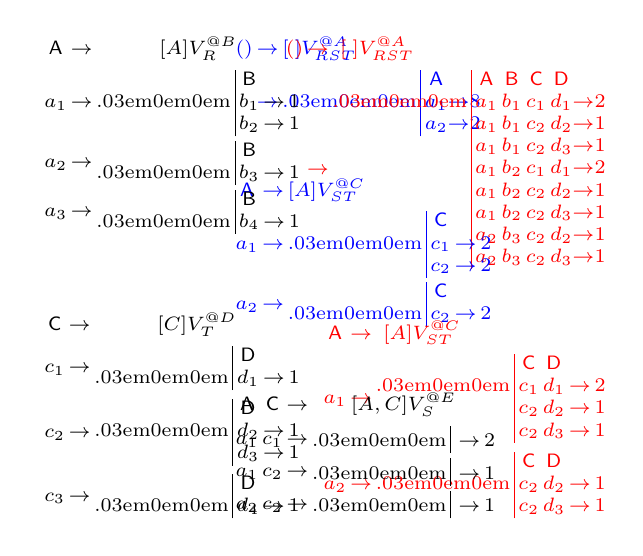
\begin{tikzpicture}[xscale=1.8, yscale=1.01]
  
        % factorized @A
        \node [text=blue, anchor=north west] at (3, 1) {
          \scriptsize
          \begin{tabular}{@{}l@{\,} @{\,}c@{\,}c@{\,}l@{}}
            & $()$ & $\to$ & $\VIEW[\;]{V^{@A}_{RST}}$ \\[1ex]\toprule 
             & $\tuple{}$ & $\rightarrow$ &
              \begin{tabular}{@{}l@{\,}!{\vrule width 0.03em}@{\,}c@{}c@{}c@{}}
                & $\mathsf{A}$ & & \\
                \specialrule{.03em}{0em}{0em} 
                & $a_1$ & $\rightarrow$ & $8$ \\
                & $a_2$ & $\rightarrow$ & $2$ \\
              \end{tabular}\\\bottomrule 
          \end{tabular}
        };
  
        % flat @A
        \node [text=red, anchor=north east] at (5.8, 1) {
          \scriptsize
          \begin{tabular}{@{}l@{\,}  @{\,}c@{\,}c@{\,}l@{}}
            & $()$ & $\rightarrow$ & \ $\VIEW[\;]{V^{@A}_{RST}}$ \\[1ex]\toprule
              & $\tuple{}$ & $\rightarrow$ & 
              \begin{tabular}{@{}l@{\,}!{\vrule width 0.03em}@{\,}c@{\,}c@{\,}c@{\,}c@{}c@{}c@{}}
                & $\mathsf{A}$ & $\mathsf{B}$ & $\mathsf{C}$ & $\mathsf{D}$ & & \\
                \specialrule{.03em}{0em}{0em} 
                & $a_1$ & $b_1$ & $c_1$ & $d_1$ & $\rightarrow$ & $2$ \\
                & $a_1$ & $b_1$ & $c_2$ & $d_2$ & $\rightarrow$ & $1$ \\
                & $a_1$ & $b_1$ & $c_2$ & $d_3$ & $\rightarrow$ & $1$ \\
                & $a_1$ & $b_2$ & $c_1$ & $d_1$ & $\rightarrow$ & $2$ \\
                & $a_1$ & $b_2$ & $c_2$ & $d_2$ & $\rightarrow$ & $1$ \\
                & $a_1$ & $b_2$ & $c_2$ & $d_3$ & $\rightarrow$ & $1$ \\
                & $a_2$ & $b_3$ & $c_2$ & $d_2$ & $\rightarrow$ & $1$ \\
                & $a_2$ & $b_3$ & $c_2$ & $d_3$ & $\rightarrow$ & $1$ \\
              \end{tabular}\\\bottomrule
          \end{tabular}
        };
  
        % factorized @C
        \node [text=blue, anchor=north west] at (3, -0.78) {
          \scriptsize
          \begin{tabular}{@{}l@{\,} @{\,}c@{\,}c@{\,}l@{}}
            & $\mathsf{A}$ & $\rightarrow$ & $\VIEW[A]{V^{@C}_{ST}}$ \\[1ex]\toprule
             & $a_1$ & $\rightarrow$ &
              \begin{tabular}{@{}l@{\,}!{\vrule width 0.03em}@{\,}c@{\,}c@{\,}c@{}}
                & $\mathsf{C}$ & & \\
                \specialrule{.03em}{0em}{0em} 
                & $c_1$ & $\rightarrow$ & $2$ \\
                & $c_2$ & $\rightarrow$ & $2$ \\
              \end{tabular} \\
            \rule{0mm}{4mm} & $a_2$ & $\rightarrow$ &
              \begin{tabular}{@{}l@{\,}!{\vrule width 0.03em}@{\,}c@{\,}c@{\,}c@{}}
                  & $\mathsf{C}$ & & \\
                  \specialrule{.03em}{0em}{0em} 
                  & $c_2$ & $\rightarrow$ & $2$ \\
              \end{tabular}\\\bottomrule 
          \end{tabular}
        };
  
        % flat @C
        \node [text=red, anchor=south east] at (5.8, -5.3) {
          \scriptsize
          \begin{tabular}{@{}l@{\,} @{\,}c@{\,}c@{\,}l@{}}
            & $\mathsf{A}$ & $\to$ & \ $\VIEW[A]{V^{@C}_{ST}}$ \\[1ex]\toprule
             & $a_1$ & $\rightarrow$ & 
              \begin{tabular}{@{}l@{\,}!{\vrule width 0.03em}@{\,}c@{\,}c@{\,}c@{\,}c@{}}
                & $\mathsf{C}$ & $\mathsf{D}$ & & \\
                \specialrule{.03em}{0em}{0em} 
                & $c_1$ & $d_1$ & $\rightarrow$ & $2$ \\
                & $c_2$ & $d_2$ & $\rightarrow$ & $1$ \\
                & $c_2$ & $d_3$ & $\rightarrow$ & $1$ \\
              \end{tabular}\\
            \rule{0mm}{6mm} & $a_2$ & $\rightarrow$ & 
              \begin{tabular}{@{}l@{\,}!{\vrule width 0.03em}@{\,}c@{\,}c@{\,}c@{\,}c@{}}
                  & $\mathsf{C}$ & $\mathsf{D}$ & & \\
                  \specialrule{.03em}{0em}{0em} 
                  & $c_2$ & $d_2$ & $\rightarrow$ & $1$ \\
                  & $c_2$ & $d_3$ & $\rightarrow$ & $1$ \\
              \end{tabular}\\\bottomrule
          \end{tabular}
        };
  
        % flat/factorized @E
        \node [anchor=south west] at (3, -5.3) {
          \scriptsize
          \begin{tabular}{@{}l@{\,} @{\,}c@{\,}c@{\,}c@{\,}c@{}}
            %  
            & $\mathsf{A}$ & $\mathsf{C}$ & $\to$ & $\VIEW[A,C]{V^{@E}_{S}}$ \\[1ex]\toprule
             & $a_1$ & $c_1$ & $\rightarrow$ & 
              \begin{tabular}{@{}l@{\,}!{\vrule width 0.03em}@{\,}c@{\,}c@{\,}c@{}}
                & & & \\[-2ex]
                \specialrule{.03em}{0em}{0em} 
                & $\tuple{}$ & $\rightarrow$ & $2$ \\
              \end{tabular} \\
            \rule{0mm}{3mm} & $a_1$ & $c_2$ & $\rightarrow$ & 
              \begin{tabular}{@{}l@{\,}!{\vrule width 0.03em}@{\,}c@{\,}c@{\,}c@{}}
                  & & & \\[-2ex]
                  \specialrule{.03em}{0em}{0em} 
                  & $\tuple{}$ & $\rightarrow$ & $1$ \\
              \end{tabular}\\
            \rule{0mm}{3mm} & $a_2$ & $c_2$ & $\rightarrow$ &
              \begin{tabular}{@{}l@{\,}!{\vrule width 0.03em}@{\,}c@{\,}c@{\,}c@{}}
                  & & & \\[-2ex]
                  \specialrule{.03em}{0em}{0em} 
                  & $\tuple{}$ & $\rightarrow$ & $1$ \\
              \end{tabular}\\\bottomrule
          \end{tabular}
        };
  
        % flat factorized @B
        \node [anchor=north west] at (1.65, 1) {
          \scriptsize
          \begin{tabular}{@{}l@{\,} @{\,}c@{\,}c@{\,}c@{}}
            %  
            & $\mathsf{A}$ & $\to$ & $\VIEW[A]{V^{@B}_{R}}$ \\[1ex]\toprule
             & $a_1$ & $\rightarrow$ &
              \begin{tabular}{@{}l@{\,}!{\vrule width 0.03em}@{\,}c@{\,}c@{\,}c@{}}
                & $\mathsf{B}$ & & \\
                \specialrule{.03em}{0em}{0em} 
                & $b_1$ & $\rightarrow$ & $1$ \\
                & $b_2$ & $\rightarrow$ & $1$ \\
              \end{tabular} \\
            \rule{0mm}{4mm} & $a_2$ & $\rightarrow$ &
              \begin{tabular}{@{}l@{\,}!{\vrule width 0.03em}@{\,}c@{\,}c@{\,}c@{}}
                  & $\mathsf{B}$ & & \\
                  \specialrule{.03em}{0em}{0em} 
                  & $b_3$ & $\rightarrow$ & $1$ \\
              \end{tabular} \\
            \rule{0mm}{4mm} & $a_3$ & $\rightarrow$ &
              \begin{tabular}{@{}l@{\,}!{\vrule width 0.03em}@{\,}c@{\,}c@{\,}c@{}}
                  & $\mathsf{B}$ & & \\
                  \specialrule{.03em}{0em}{0em} 
                  & $b_4$ & $\rightarrow$ & $1$ \\
              \end{tabular}\\\bottomrule 
          \end{tabular}
        };
  
        % flat/factorized @D
        \node [anchor=south west] at (1.65, -5.3) {
          \scriptsize
          \begin{tabular}{@{}l@{\,} @{\,}c@{\,}c@{\,}c@{}}
            %  
            & $\mathsf{C}$ & $\to$ & $\VIEW[C]{V^{@D}_{T}}$ \\[1ex]\toprule
             & $c_1$ & $\rightarrow$ &
              \begin{tabular}{@{}l@{\,}!{\vrule width 0.03em}@{\,}c@{\,}c@{\,}c@{}}
                  & $\mathsf{D}$ & & \\
                  \specialrule{.03em}{0em}{0em} 
                  & $d_1$ & $\rightarrow$ & $1$ \\
              \end{tabular} \\
            \rule{0mm}{6mm} & $c_2$ & $\rightarrow$ & 
              \begin{tabular}{@{}l@{\,}!{\vrule width 0.03em}@{\,}c@{\,}c@{\,}c@{}}
                & $\mathsf{D}$ & & \\
                \specialrule{.03em}{0em}{0em} 
                & $d_2$ & $\rightarrow$ & $1$ \\
                & $d_3$ & $\rightarrow$ & $1$ \\
              \end{tabular} \\
            \rule{0mm}{4.5mm} & $c_3$ & $\rightarrow$ &
              \begin{tabular}{@{}l@{\,}!{\vrule width 0.03em}@{\,}c@{\,}c@{\,}c@{}}
                  & $\mathsf{D}$ & & \\
                  \specialrule{.03em}{0em}{0em} 
                  & $d_4$ & $\rightarrow$ & $1$ \\
              \end{tabular}\\\bottomrule 
          \end{tabular}
        };
      \end{tikzpicture}
    \end{minipage}
  %}
  \caption{
  Computing the query from Example~\ref{ex:relational_ring} 
  over the database
   in Figure~\ref{fig:count} 
   and the relational ring, where $\forall i\in[12]: p_i=\{ () \to 1 \}$.
   The computation uses 
   the view tree $\tau$
  in Figure~\ref{fig:example_payloads}.
   The red views (rightmost column) have payloads storing the listing representation of the intermediate and final query results. The blue views (top two views in the middle column) encode a factorized representation of these results distributed over their payloads. The remaining (black) views remain the same for both representations.
  }
  \label{fig:factorized_listing_ring}
\end{figure}
  
  

\nop{
%%%%%%%%%%%%%%%%%%%%%%%%%%%% Figure: Example with relational and factorized payload ring
\begin{figure*}[t]
\hspace*{-12mm}
\subfloat[Database $\db$]
{
  \label{fig:example_payloads_database}
  \begin{minipage}[b]{2cm} 
    \scriptsize    
    \begin{tabular}{@{}l@{~~}l@{~$\to$~}l@{}}
      $A$ & $B$ & $\VIEW{R}[A,B]$\\\toprule
      $a_1$ & $b_1$ & $p_1$ \\
      $a_1$ & $b_2$ & $p_2$\\  
      $a_2$ & $b_3$ & $p_3$\\
      $a_3$ & $b_4$ & $p_4$\\\bottomrule
    \end{tabular}
    \\[4ex]
    \begin{tabular}{@{}l@{~~}l@{~~}l@{~$\to$~}l@{}}
      $A$ & $C$ & $E$ & $\VIEW{S}[A,C,E]$ \\\toprule
      $a_1$ & $c_1$ & $e_1$ & $p_4$\\
      $a_1$ & $c_1$ & $e_2$ & $p_5$\\
      $a_1$ & $c_2$ & $e_3$ & $p_6$\\
      $a_2$ & $c_2$ & $e_4$ & $p_7$\\\bottomrule
    \end{tabular}
    \\[4ex]
    \begin{tabular}{@{}l@{~~}l@{~$\to$~}l@{}}
      $C$ & $D$ & $\VIEW{T}[C,D]$ \\\toprule
      $c_1$ & $d_1$ & $p_9$\\
      $c_2$ & $d_2$ & $p_{10}$\\
      $c_2$ & $d_3$ & $p_{11}$\\
      $c_3$ & $d_4$ & $p_{12}$\\\bottomrule
    \end{tabular}
    \vspace{0.5em}

  \end{minipage}
}
% 
\qquad
% 
\subfloat[View tree $\tau$]
{
  \label{fig:example_payloads_viewtree}
  \begin{minipage}[b]{4.5cm}
    \small
    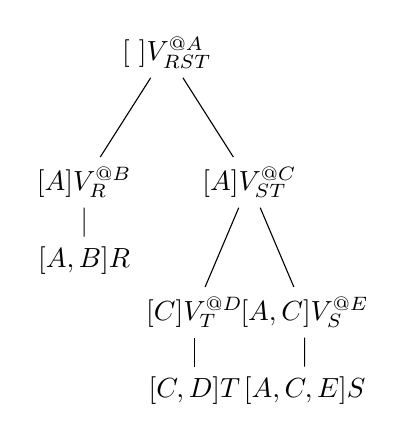
\begin{tikzpicture}[xscale=0.7, yscale=0.33]

      \node at (0, 0) (A) {$\VIEW[~]{V^{@A}_{RST}}$};
      \node at (-1.5, -5) (B) {$\VIEW[A]{V^{@B}_{R}}$} edge[-] (A);
      \node at (1.5, -5) (C) {$\VIEW[A]{V^{@C}_{ST}}$} edge[-] (A);
      \node at (0.5, -10) (D) {$\VIEW[C]{V^{@D}_{T}}$} edge[-] (C);
      \node at (2.5, -10) (E) {$\VIEW[A,C]{V^{@E}_{S}}$} edge[-] (C);
      
      \node at (-1.5, -8) {$\VIEW[A,B]{R}$} edge[-] (B);
      \node at (2.5, -13) {$\VIEW[A,C,E]{S}$} edge[-] (E);
      \node at (0.5, -13) {$\VIEW[C,D]{T}$} edge[-] (D);

    \end{tikzpicture}
    \vspace{0.5em}

  \end{minipage}  
}
% 
\qquad
%
\subfloat[{\tt COUNT} query]
{
  \label{fig:example_payloads_count}
  \begin{minipage}[b]{3.5cm}
    \scriptsize
    \hspace*{-2em}
    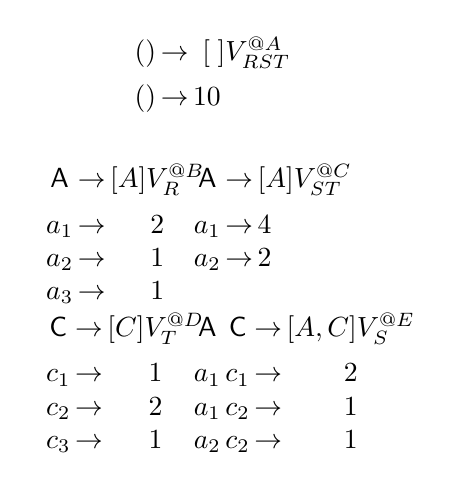
\begin{tikzpicture}[xscale=0.75, yscale=0.27]
      % at node A
      \node [anchor=north west] at (-5, 9) {
        \begin{tabular}{@{}l@{\,}  @{\,}c@{\,}c@{\,}l@{}}
          & $()$ & $\rightarrow$ & \ $\VIEW[\;]{V^{@A}_{RST}}$ \\[1ex]\toprule
          & $()$ & $\rightarrow$ & 10 \\\bottomrule
        \end{tabular}
      };

      % at node B
      \node [anchor=north west] at (-6.5, 3) {
        \begin{tabular}{@{}l@{\,} @{\,}c@{\,}c@{\,}c@{}}
          %  
          & $\mathsf{A}$ & $\to$ & $\VIEW[A]{V^{@B}_{R}}$ \\[1ex]\toprule
          & $a_1$ & $\rightarrow$ & 2 \\
          & $a_2$ & $\rightarrow$ & 1 \\
          & $a_3$ & $\rightarrow$ & 1\\\bottomrule
        \end{tabular}
      };

      % at node C
      \node [anchor=north west] at (-4, 3) {
        \begin{tabular}{@{}l@{\,} @{\,}c@{\,}c@{\,}l@{}}
          & $\mathsf{A}$ & $\rightarrow$ & $\VIEW[A]{V^{@C}_{ST}}$ \\[1ex]\toprule
          & $a_1$ & $\rightarrow$ & 4 \\
          & $a_2$ & $\rightarrow$ & 2 \\\bottomrule 
        \end{tabular}
      };

      % at node D
      \node [anchor=north west] at (-6.5, -4) {
        \begin{tabular}{@{}l@{\,} @{\,}c@{\,}c@{\,}c@{}}
          %  
          & $\mathsf{C}$ & $\to$ & $\VIEW[C]{V^{@D}_{T}}$ \\[1ex]\toprule
          & $c_1$ & $\rightarrow$ & 1 \\
          & $c_2$ & $\rightarrow$ & 2 \\
          & $c_3$ & $\rightarrow$ & 1 \\\bottomrule
        \end{tabular}
      };

      % at node E
      \node [anchor=north west] at (-4, -4) {
        \begin{tabular}{@{}l@{\,} @{\,}c@{\,}c@{\,}c@{\,}c@{}}
          & $\mathsf{A}$ & $\mathsf{C}$ & $\to$ & $\VIEW[A,C]{V^{@E}_{S}}$ \\[1ex]\toprule
          & $a_1$ & $c_1$ & $\rightarrow$ & 2 \\
          & $a_1$ & $c_2$ & $\rightarrow$ & 1 \\
          & $a_2$ & $c_2$ & $\rightarrow$ & 1 \\\bottomrule
        \end{tabular}
      };

    \end{tikzpicture}
    \vspace{-1em}

  \end{minipage}
}
% 
\quad
% 
\subfloat[Conjunctive query]
{
  \label{fig:example_payloads_conjunctive}
  \scalebox{0.9}{
  \begin{minipage}[b]{5cm}
    \centering
    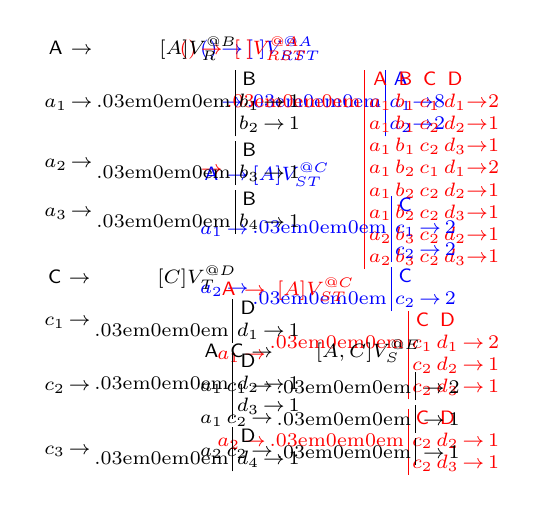
\begin{tikzpicture}[xscale=1.8, yscale=0.9]

      % factorized @A
      \node [text=blue, anchor=north west] at (2.4, 1) {
        \scriptsize
        \begin{tabular}{@{}l@{\,} @{\,}c@{\,}c@{\,}l@{}}
          & $()$ & $\to$ & $\VIEW[\;]{V^{@A}_{RST}}$ \\[1ex]\toprule 
           & $\tuple{}$ & $\rightarrow$ &
            \begin{tabular}{@{}l@{\,}!{\vrule width 0.03em}@{\,}c@{}c@{}c@{}}
              & $\mathsf{A}$ & & \\
              \specialrule{.03em}{0em}{0em} 
              & $a_1$ & $\rightarrow$ & $8$ \\
              & $a_2$ & $\rightarrow$ & $2$ \\
            \end{tabular}\\\bottomrule 
        \end{tabular}
      };

      % flat @A
      \node [text=red, anchor=north east] at (4.7, 1) {
        \scriptsize
        \begin{tabular}{@{}l@{\,}  @{\,}c@{\,}c@{\,}l@{}}
          & $()$ & $\rightarrow$ & \ $\VIEW[\;]{V^{@A}_{RST}}$ \\[1ex]\toprule
            & $\tuple{}$ & $\rightarrow$ & 
            \begin{tabular}{@{}l@{\,}!{\vrule width 0.03em}@{\,}c@{\,}c@{\,}c@{\,}c@{}c@{}c@{}}
              & $\mathsf{A}$ & $\mathsf{B}$ & $\mathsf{C}$ & $\mathsf{D}$ & & \\
              \specialrule{.03em}{0em}{0em} 
              & $a_1$ & $b_1$ & $c_1$ & $d_1$ & $\rightarrow$ & $2$ \\
              & $a_1$ & $b_1$ & $c_2$ & $d_2$ & $\rightarrow$ & $1$ \\
              & $a_1$ & $b_1$ & $c_2$ & $d_3$ & $\rightarrow$ & $1$ \\
              & $a_1$ & $b_2$ & $c_1$ & $d_1$ & $\rightarrow$ & $2$ \\
              & $a_1$ & $b_2$ & $c_2$ & $d_2$ & $\rightarrow$ & $1$ \\
              & $a_1$ & $b_2$ & $c_2$ & $d_3$ & $\rightarrow$ & $1$ \\
              & $a_2$ & $b_3$ & $c_2$ & $d_2$ & $\rightarrow$ & $1$ \\
              & $a_2$ & $b_3$ & $c_2$ & $d_3$ & $\rightarrow$ & $1$ \\
            \end{tabular}\\\bottomrule
        \end{tabular}
      };

      % factorized @C
      \node [text=blue, anchor=north west] at (2.4, -0.78) {
        \scriptsize
        \begin{tabular}{@{}l@{\,} @{\,}c@{\,}c@{\,}l@{}}
          & $\mathsf{A}$ & $\rightarrow$ & $\VIEW[A]{V^{@C}_{ST}}$ \\[1ex]\toprule
           & $a_1$ & $\rightarrow$ &
            \begin{tabular}{@{}l@{\,}!{\vrule width 0.03em}@{\,}c@{\,}c@{\,}c@{}}
              & $\mathsf{C}$ & & \\
              \specialrule{.03em}{0em}{0em} 
              & $c_1$ & $\rightarrow$ & $2$ \\
              & $c_2$ & $\rightarrow$ & $2$ \\
            \end{tabular} \\
          \rule{0mm}{4mm} & $a_2$ & $\rightarrow$ &
            \begin{tabular}{@{}l@{\,}!{\vrule width 0.03em}@{\,}c@{\,}c@{\,}c@{}}
                & $\mathsf{C}$ & & \\
                \specialrule{.03em}{0em}{0em} 
                & $c_2$ & $\rightarrow$ & $2$ \\
            \end{tabular}\\\bottomrule 
        \end{tabular}
      };

      % flat @C
      \node [text=red, anchor=north east] at (4.7, -2.4) {
        \scriptsize
        \begin{tabular}{@{}l@{\,} @{\,}c@{\,}c@{\,}l@{}}
          & $\mathsf{A}$ & $\to$ & \ $\VIEW[A]{V^{@C}_{ST}}$ \\[1ex]\toprule
           & $a_1$ & $\rightarrow$ & 
            \begin{tabular}{@{}l@{\,}!{\vrule width 0.03em}@{\,}c@{\,}c@{\,}c@{\,}c@{}}
              & $\mathsf{C}$ & $\mathsf{D}$ & & \\
              \specialrule{.03em}{0em}{0em} 
              & $c_1$ & $d_1$ & $\rightarrow$ & $2$ \\
              & $c_2$ & $d_2$ & $\rightarrow$ & $1$ \\
              & $c_2$ & $d_3$ & $\rightarrow$ & $1$ \\
            \end{tabular}\\
          \rule{0mm}{6mm} & $a_2$ & $\rightarrow$ & 
            \begin{tabular}{@{}l@{\,}!{\vrule width 0.03em}@{\,}c@{\,}c@{\,}c@{\,}c@{}}
                & $\mathsf{C}$ & $\mathsf{D}$ & & \\
                \specialrule{.03em}{0em}{0em} 
                & $c_2$ & $d_2$ & $\rightarrow$ & $1$ \\
                & $c_2$ & $d_3$ & $\rightarrow$ & $1$ \\
            \end{tabular}\\\bottomrule
        \end{tabular}
      };

      % flat/factorized @E
      \node [anchor=north west] at (2.4, -3.27) {
        \scriptsize
        \begin{tabular}{@{}l@{\,} @{\,}c@{\,}c@{\,}c@{\,}c@{}}
          %  
          & $\mathsf{A}$ & $\mathsf{C}$ & $\to$ & $\VIEW[A,C]{V^{@E}_{S}}$ \\[1ex]\toprule
           & $a_1$ & $c_1$ & $\rightarrow$ & 
            \begin{tabular}{@{}l@{\,}!{\vrule width 0.03em}@{\,}c@{\,}c@{\,}c@{}}
              & & & \\[-2ex]
              \specialrule{.03em}{0em}{0em} 
              & $\tuple{}$ & $\rightarrow$ & $2$ \\
            \end{tabular} \\
          \rule{0mm}{3mm} & $a_1$ & $c_2$ & $\rightarrow$ & 
            \begin{tabular}{@{}l@{\,}!{\vrule width 0.03em}@{\,}c@{\,}c@{\,}c@{}}
                & & & \\[-2ex]
                \specialrule{.03em}{0em}{0em} 
                & $\tuple{}$ & $\rightarrow$ & $1$ \\
            \end{tabular}\\
          \rule{0mm}{3mm} & $a_2$ & $c_2$ & $\rightarrow$ &
            \begin{tabular}{@{}l@{\,}!{\vrule width 0.03em}@{\,}c@{\,}c@{\,}c@{}}
                & & & \\[-2ex]
                \specialrule{.03em}{0em}{0em} 
                & $\tuple{}$ & $\rightarrow$ & $1$ \\
            \end{tabular}\\\bottomrule
        \end{tabular}
      };

      % flat factorized @B
      \node [anchor=north west] at (1.3, 1) {
        \scriptsize
        \begin{tabular}{@{}l@{\,} @{\,}c@{\,}c@{\,}c@{}}
          %  
          & $\mathsf{A}$ & $\to$ & $\VIEW[A]{V^{@B}_{R}}$ \\[1ex]\toprule
           & $a_1$ & $\rightarrow$ &
            \begin{tabular}{@{}l@{\,}!{\vrule width 0.03em}@{\,}c@{\,}c@{\,}c@{}}
              & $\mathsf{B}$ & & \\
              \specialrule{.03em}{0em}{0em} 
              & $b_1$ & $\rightarrow$ & $1$ \\
              & $b_2$ & $\rightarrow$ & $1$ \\
            \end{tabular} \\
          \rule{0mm}{4mm} & $a_2$ & $\rightarrow$ &
            \begin{tabular}{@{}l@{\,}!{\vrule width 0.03em}@{\,}c@{\,}c@{\,}c@{}}
                & $\mathsf{B}$ & & \\
                \specialrule{.03em}{0em}{0em} 
                & $b_3$ & $\rightarrow$ & $1$ \\
            \end{tabular} \\
          \rule{0mm}{4mm} & $a_3$ & $\rightarrow$ &
            \begin{tabular}{@{}l@{\,}!{\vrule width 0.03em}@{\,}c@{\,}c@{\,}c@{}}
                & $\mathsf{B}$ & & \\
                \specialrule{.03em}{0em}{0em} 
                & $b_4$ & $\rightarrow$ & $1$ \\
            \end{tabular}\\\bottomrule 
        \end{tabular}
      };

      % flat/factorized @D
      \node [anchor=north west] at (1.3, -2.23) {
        \scriptsize
        \begin{tabular}{@{}l@{\,} @{\,}c@{\,}c@{\,}c@{}}
          %  
          & $\mathsf{C}$ & $\to$ & $\VIEW[C]{V^{@D}_{T}}$ \\[1ex]\toprule
           & $c_1$ & $\rightarrow$ &
            \begin{tabular}{@{}l@{\,}!{\vrule width 0.03em}@{\,}c@{\,}c@{\,}c@{}}
                & $\mathsf{D}$ & & \\
                \specialrule{.03em}{0em}{0em} 
                & $d_1$ & $\rightarrow$ & $1$ \\
            \end{tabular} \\
          \rule{0mm}{6mm} & $c_2$ & $\rightarrow$ & 
            \begin{tabular}{@{}l@{\,}!{\vrule width 0.03em}@{\,}c@{\,}c@{\,}c@{}}
              & $\mathsf{D}$ & & \\
              \specialrule{.03em}{0em}{0em} 
              & $d_2$ & $\rightarrow$ & $1$ \\
              & $d_3$ & $\rightarrow$ & $1$ \\
            \end{tabular} \\
          \rule{0mm}{4.5mm} & $c_3$ & $\rightarrow$ &
            \begin{tabular}{@{}l@{\,}!{\vrule width 0.03em}@{\,}c@{\,}c@{\,}c@{}}
                & $\mathsf{D}$ & & \\
                \specialrule{.03em}{0em}{0em} 
                & $d_4$ & $\rightarrow$ & $1$ \\
            \end{tabular}\\\bottomrule 
        \end{tabular}
      };

    \end{tikzpicture}

  \end{minipage}
  }
}

\caption{ 
(a) Database $\db$ with relations $\VIEW{R}$, $\VIEW{S}$, $\VIEW{T}$ over a ring $\RING$, where $\{p_i\}_{i\in[12]}\subseteq\RING$. 
(b) View tree $\tau$ for a query without free variables. 
(c) Computing the {\tt COUNT} query using $\tau$ and the $\mathbb{Z}$ ring, where $\forall i\in[12]: p_i=1$. 
(d) Computing the query from Example~\ref{ex:relational_ring} using $\tau$ and the relational ring, where $\forall i\in[12]: p_i=\{ () \to 1 \}$. The red views (rightmost column) have payloads storing the listing representation of the intermediate and final query results. The blue views (middle) encode a factorized representation of these results distributed over their payloads. The black views remain the same for both representations.
}
\label{fig:example_payloads}\vspace*{-1em}
\end{figure*}
}

\nop{
\begin{figure}
  \centering
  \hspace*{-2mm}
  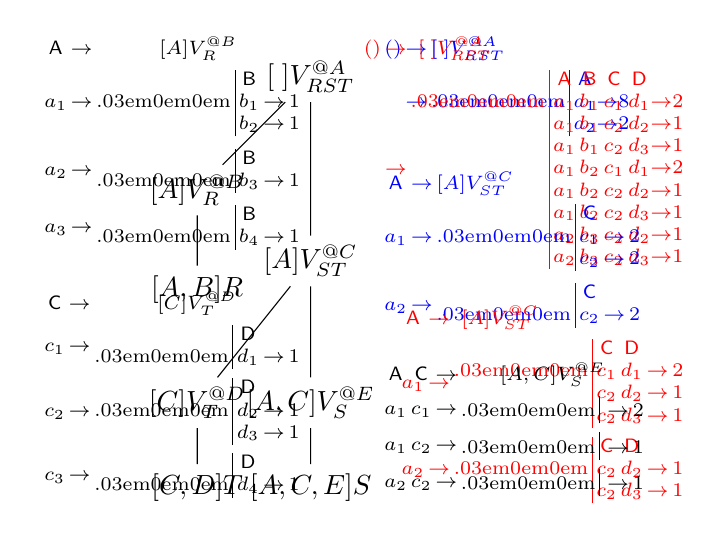
\begin{tikzpicture}[xscale=1.8, yscale=0.9]

    \node at (2, 0.3) (A) {$\VIEW[\;]{V^{@A}_{RST}}$};
    \node at (1.2, -1.3) (B) {$\VIEW[A]{V^{@B}_{R}}$} edge[-] (A);
    \node at (2, -2.3) (C) {$\VIEW[A]{V^{@C}_{ST}}$} edge[-] (A);
    \node at (1.2, -4.3) (D) {$\VIEW[C]{V^{@D}_{T}}$} edge[-] (C);
    \node at (2, -4.3) (E) {$\VIEW[A,C]{V^{@E}_{S}}$} edge[-] (C);
    
    \node at (1.2, -2.7) {$\VIEW[A,B]{R}$} edge[-] (B);
    \node at (2, -5.5) {$\VIEW[A,C,E]{S}$} edge[-] (E);
    \node at (1.2, -5.5) {$\VIEW[C,D]{T}$} edge[-] (D);

    % factorized @A
    \node [text=blue, anchor=north west] at (2.4, 1) {
      \scriptsize
      \begin{tabular}{@{}l@{\,} @{\,}c@{\,}c@{\,}l@{}}
        & $()$ & $\to$ & $\VIEW[\;]{V^{@A}_{RST}}$ \\[1ex]\toprule 
         & $\tuple{}$ & $\rightarrow$ &
          \begin{tabular}{@{}l@{\,}!{\vrule width 0.03em}@{\,}c@{}c@{}c@{}}
            & $\mathsf{A}$ & & \\
            \specialrule{.03em}{0em}{0em} 
            & $a_1$ & $\rightarrow$ & $8$ \\
            & $a_2$ & $\rightarrow$ & $2$ \\
          \end{tabular}\\\bottomrule 
      \end{tabular}
    };

    % flat @A
    \node [text=red, anchor=north east] at (4.7, 1) {
      \scriptsize
      \begin{tabular}{@{}l@{\,}  @{\,}c@{\,}c@{\,}l@{}}
        & $()$ & $\rightarrow$ & \ $\VIEW[\;]{V^{@A}_{RST}}$ \\[1ex]\toprule
          & $\tuple{}$ & $\rightarrow$ & 
          \begin{tabular}{@{}l@{\,}!{\vrule width 0.03em}@{\,}c@{\,}c@{\,}c@{\,}c@{}c@{}c@{}}
            & $\mathsf{A}$ & $\mathsf{B}$ & $\mathsf{C}$ & $\mathsf{D}$ & & \\
            \specialrule{.03em}{0em}{0em} 
            & $a_1$ & $b_1$ & $c_1$ & $d_1$ & $\rightarrow$ & $2$ \\
            & $a_1$ & $b_1$ & $c_2$ & $d_2$ & $\rightarrow$ & $1$ \\
            & $a_1$ & $b_1$ & $c_2$ & $d_3$ & $\rightarrow$ & $1$ \\
            & $a_1$ & $b_2$ & $c_1$ & $d_1$ & $\rightarrow$ & $2$ \\
            & $a_1$ & $b_2$ & $c_2$ & $d_2$ & $\rightarrow$ & $1$ \\
            & $a_1$ & $b_2$ & $c_2$ & $d_3$ & $\rightarrow$ & $1$ \\
            & $a_2$ & $b_3$ & $c_2$ & $d_2$ & $\rightarrow$ & $1$ \\
            & $a_2$ & $b_3$ & $c_2$ & $d_3$ & $\rightarrow$ & $1$ \\
          \end{tabular}\\\bottomrule
      \end{tabular}
    };

    % factorized @C
    \node [text=blue, anchor=north west] at (2.4, -0.9) {
      \scriptsize
      \begin{tabular}{@{}l@{\,} @{\,}c@{\,}c@{\,}l@{}}
        & $\mathsf{A}$ & $\rightarrow$ & $\VIEW[A]{V^{@C}_{ST}}$ \\[1ex]\toprule
         & $a_1$ & $\rightarrow$ &
          \begin{tabular}{@{}l@{\,}!{\vrule width 0.03em}@{\,}c@{\,}c@{\,}c@{}}
            & $\mathsf{C}$ & & \\
            \specialrule{.03em}{0em}{0em} 
            & $c_1$ & $\rightarrow$ & $2$ \\
            & $c_2$ & $\rightarrow$ & $2$ \\
          \end{tabular} \\
        \rule{0mm}{5mm} & $a_2$ & $\rightarrow$ &
          \begin{tabular}{@{}l@{\,}!{\vrule width 0.03em}@{\,}c@{\,}c@{\,}c@{}}
              & $\mathsf{C}$ & & \\
              \specialrule{.03em}{0em}{0em} 
              & $c_2$ & $\rightarrow$ & $2$ \\
          \end{tabular}\\\bottomrule 
      \end{tabular}
    };

    % flat @C
    \node [text=red, anchor=north east] at (4.7, -2.8) {
      \scriptsize
      \begin{tabular}{@{}l@{\,} @{\,}c@{\,}c@{\,}l@{}}
        & $\mathsf{A}$ & $\to$ & \ $\VIEW[A]{V^{@C}_{ST}}$ \\[1ex]\toprule
         & $a_1$ & $\rightarrow$ & 
          \begin{tabular}{@{}l@{\,}!{\vrule width 0.03em}@{\,}c@{\,}c@{\,}c@{\,}c@{}}
            & $\mathsf{C}$ & $\mathsf{D}$ & & \\
            \specialrule{.03em}{0em}{0em} 
            & $c_1$ & $d_1$ & $\rightarrow$ & $2$ \\
            & $c_2$ & $d_2$ & $\rightarrow$ & $1$ \\
            & $c_2$ & $d_3$ & $\rightarrow$ & $1$ \\
          \end{tabular}\\
        \rule{0mm}{6mm} & $a_2$ & $\rightarrow$ & 
          \begin{tabular}{@{}l@{\,}!{\vrule width 0.03em}@{\,}c@{\,}c@{\,}c@{\,}c@{}}
              & $\mathsf{C}$ & $\mathsf{D}$ & & \\
              \specialrule{.03em}{0em}{0em} 
              & $c_2$ & $d_2$ & $\rightarrow$ & $1$ \\
              & $c_2$ & $d_3$ & $\rightarrow$ & $1$ \\
          \end{tabular}\\\bottomrule
      \end{tabular}
    };

    % flat/factorized @E
    \node [anchor=north west] at (2.4, -3.6) {
      \scriptsize
      \begin{tabular}{@{}l@{\,} @{\,}c@{\,}c@{\,}c@{\,}c@{}}
        %  
        & $\mathsf{A}$ & $\mathsf{C}$ & $\to$ & $\VIEW[A,C]{V^{@E}_{S}}$ \\[1ex]\toprule
         & $a_1$ & $c_1$ & $\rightarrow$ & 
          \begin{tabular}{@{}l@{\,}!{\vrule width 0.03em}@{\,}c@{\,}c@{\,}c@{}}
            & & & \\[-2ex]
            \specialrule{.03em}{0em}{0em} 
            & $\tuple{}$ & $\rightarrow$ & $2$ \\
          \end{tabular} \\
        \rule{0mm}{3.5mm} & $a_1$ & $c_2$ & $\rightarrow$ & 
          \begin{tabular}{@{}l@{\,}!{\vrule width 0.03em}@{\,}c@{\,}c@{\,}c@{}}
              & & & \\[-2ex]
              \specialrule{.03em}{0em}{0em} 
              & $\tuple{}$ & $\rightarrow$ & $1$ \\
          \end{tabular}\\
        \rule{0mm}{3.5mm} & $a_2$ & $c_2$ & $\rightarrow$ &
          \begin{tabular}{@{}l@{\,}!{\vrule width 0.03em}@{\,}c@{\,}c@{\,}c@{}}
              & & & \\[-2ex]
              \specialrule{.03em}{0em}{0em} 
              & $\tuple{}$ & $\rightarrow$ & $1$ \\
          \end{tabular}\\\bottomrule
      \end{tabular}
    };

    % flat factorized @B
    \node [anchor=north west] at (0, 1) {
      \scriptsize
      \begin{tabular}{@{}l@{\,} @{\,}c@{\,}c@{\,}c@{}}
        %  
        & $\mathsf{A}$ & $\to$ & $\VIEW[A]{V^{@B}_{R}}$ \\[1ex]\toprule
         & $a_1$ & $\rightarrow$ &
          \begin{tabular}{@{}l@{\,}!{\vrule width 0.03em}@{\,}c@{\,}c@{\,}c@{}}
            & $\mathsf{B}$ & & \\
            \specialrule{.03em}{0em}{0em} 
            & $b_1$ & $\rightarrow$ & $1$ \\
            & $b_2$ & $\rightarrow$ & $1$ \\
          \end{tabular} \\
        \rule{0mm}{5mm} & $a_2$ & $\rightarrow$ &
          \begin{tabular}{@{}l@{\,}!{\vrule width 0.03em}@{\,}c@{\,}c@{\,}c@{}}
              & $\mathsf{B}$ & & \\
              \specialrule{.03em}{0em}{0em} 
              & $b_3$ & $\rightarrow$ & $1$ \\
          \end{tabular} \\
        \rule{0mm}{5mm} & $a_3$ & $\rightarrow$ &
          \begin{tabular}{@{}l@{\,}!{\vrule width 0.03em}@{\,}c@{\,}c@{\,}c@{}}
              & $\mathsf{B}$ & & \\
              \specialrule{.03em}{0em}{0em} 
              & $b_4$ & $\rightarrow$ & $1$ \\
          \end{tabular}\\\bottomrule 
      \end{tabular}
    };

    % flat/factorized @D
    \node [anchor=north west] at (0, -2.6) {
      \scriptsize
      \begin{tabular}{@{}l@{\,} @{\,}c@{\,}c@{\,}c@{}}
        %  
        & $\mathsf{C}$ & $\to$ & $\VIEW[C]{V^{@D}_{T}}$ \\[1ex]\toprule
         & $c_1$ & $\rightarrow$ &
          \begin{tabular}{@{}l@{\,}!{\vrule width 0.03em}@{\,}c@{\,}c@{\,}c@{}}
              & $\mathsf{D}$ & & \\
              \specialrule{.03em}{0em}{0em} 
              & $d_1$ & $\rightarrow$ & $1$ \\
          \end{tabular} \\
        \rule{0mm}{6mm} & $c_2$ & $\rightarrow$ & 
          \begin{tabular}{@{}l@{\,}!{\vrule width 0.03em}@{\,}c@{\,}c@{\,}c@{}}
            & $\mathsf{D}$ & & \\
            \specialrule{.03em}{0em}{0em} 
            & $d_2$ & $\rightarrow$ & $1$ \\
            & $d_3$ & $\rightarrow$ & $1$ \\
          \end{tabular} \\
        \rule{0mm}{4.5mm} & $c_3$ & $\rightarrow$ &
          \begin{tabular}{@{}l@{\,}!{\vrule width 0.03em}@{\,}c@{\,}c@{\,}c@{}}
              & $\mathsf{D}$ & & \\
              \specialrule{.03em}{0em}{0em} 
              & $d_4$ & $\rightarrow$ & $1$ \\
          \end{tabular}\\\bottomrule 
      \end{tabular}
    };

  \end{tikzpicture}
\caption{Computing the query in Example~\ref{ex:relational_ring}. The red views (rightmost column) have payloads storing the listing representation of the intermediate and final query results. The blue views (middle) encode a factorized representation of these results distributed over their payloads. The black views  remain the same for both representations.}
\label{fig:example_payloads_conjunctive}\vspace*{-1.5em}
\end{figure}
}
%%%%%%%%%%%%%%%%%%%%%%%%%%%%
We next show how to construct a factorized representation of the query result. In contrast to the scenarios discussed above, this representation is {\em not} available as one payload at the root view, but {\em distributed} over the payloads of all views. This hierarchy of payloads, linked via the keys of the views, becomes the factorized representation. A further difference lies with the multiplication operation. For the listing representation, the multiplication is the Cartesian product. For a given view, it is used to concatenate payloads from its child views. For the factorized representation, we further project away values for all but the marginalized variable. More precisely, for each view $\VIEW[\mathcal{S}]{V^{@X}_{rels}}$ and each of its keys $a_{\mathcal{S}}$, let $\VIEW[\mathcal{T}]{P} = \VIEW[a_\mathcal{S}]{V^{@X}_{rels}}$ be the corresponding payload relation. Then, instead of computing this payload, we compute $\VSUM_{Y\in \mathcal{T}-\{X\}}\VIEW[\mathcal{T}]{P}$ by marginalizing the variables in $\mathcal{T}-\{X\}$ and summing up the multiplicities of the tuples in $\VIEW[\mathcal{T}]{P}$ with the same $X$-value.

\begin{example}
\label{ex:factorized_ring}
We continue Example~\ref{ex:relational_ring}. 
Figure~\ref{fig:factorized_listing_ring} shows the contents of the views with factorized payloads (first two columns in black and blue). 
Each view stores relational payloads that have the schema of the marginalized variable. 
Together, these payloads form a factorized representation over the variable order $\omega$ used to define the view tree in Figure~\ref{fig:example_payloads}. At the top of the factorization, we have a union of two $A$-values: $a_1$ and $a_2$. This is stored in the payloads of (middle) {\color{blue}$\VIEW[\;]{V^{A}_{RST}}$}. The payloads of (middle) {\color{blue}$\VIEW[A]{V^{@C}_{ST}}$} store a union of $C$-values $c_1$ and $c_2$ under $a_1$, and a singleton union of $c_2$ under $a_2$. The payloads of $\VIEW[A]{V^{@B}_R}$ store a union of $B$-values $b_1$ and $b_2$ under $a_1$ and a singleton union of $b_3$ under $a_2$. Note the (conditional) independence of the variables $B$ and $C$ given a value for $A$. This is key to succinctness of factorization. In contrast, the listing representation explicitly materializes all pairings of $B$ and $C$-values for each $A$-value, as shown in the payload of (right) {\color{red}$\VIEW[\;]{V^{A}_{RST}}$}. Furthermore, the variable $D$ is independent of the other variables {\em given} $C$. This is a further source of succinctness in the factorization: Even though $c_2$ occurs under both $a_1$ and $a_2$, the relations under $c_2$, in this case the union of $d_2$ and $d_3$, is only stored once in $\VIEW[C]{V^{@D}_T}$. Each value in the factorization keeps a multiplicity, that is, the number of its derivations from the input data. This is necessary for maintenance. 

This factorization is over a variable order that can be used for all queries with same body and different free variables: As long as their free variables sit on top of the bound variables, the variable order is valid and so is the factorization over it. For instance, if the variable $D$ were not free,  then the factorization for the new query would be the same except that we would now discard the $D$-values from the payload of the view $\VIEW{V^{@D}_{T}}$.\punto
\end{example}


%%%%%%%%%%%%%%%%%%%%%%%%%%%%

\subsection{Matrix Chain Multiplication}
\label{sec:mcm}

Consider the problem of computing a product of a sequence of matrices $\bm{A}_1, \ldots, \bm{A}_n$ over some ring $\RING$, where matrix $\bm{A}_i[x_i, x_{i+1}]$ has the size $p_{i} \times p_{i+1}$, $i \in [n]$. The product $\bm{A} = \bm{A}_1 \cdots \bm{A}_n$ is a matrix of size $p_1 \times p_{n+1}$ and can be formulated as follows:

\begin{align*}
\bm{A}[x_1, x_{n+1}] = \sum_{x_2 \in[p_2]} \cdots \sum_{x_n\in [p_n]} \prod_{i\in[n]} \bm{A}_i[x_i, x_{i+1}]
\end{align*}

We model a matrix $\bm{A}_i$ as a relation $\VIEW[X_i, X_{i+1}]{A_i}$ with the payload carrying matrix values. The query that computes the matrix $\bm{A}$ is:
\begin{align*}
\VIEW[X_1, X_{n+1}]{A} = \VSUM_{X_2} \cdots \VSUM_{X_n} \VPRODBIG_{i \in [n]} \VIEW[X_i, X_{i+1}]{A_i}
\end{align*}
where each of the lifting functions $\{g_{X_j}\}_{j \in [2,n]}$ maps any key value to payload $\RINGONE\in\RING$.
Different variable orders lead to different evaluation plans for matrix chain multiplication. The optimal variable order corresponds to the optimal sequence of matrix multiplications that minimizes the overall multiplication cost, which is the textbook Matrix Chain Multiplication problem~\cite{Cormen:2009:Algorithms}.

\begin{example}
\label{ex:MCM-factorized-update}
Consider a multiplication chain of $4$ matrices of equal size $p \times p$ encoded as relations $\VIEW[X_i, X_{i+1}]{A_i}$. Let $\mathcal{F} = \{ X_1, X_5 \}$ be the set of free variables and $\omega$ be the variable order $X_1 - X_5 - X_3 - \{ X_2, X_4 \}$, i.e., $X_2$ and $X_4$ are children of $X_3$, with the matrix relations placed below the leaf variables in $\omega$. The view tree $\tau(\omega, \mathcal{F})$ has the following views (from bottom to top; the views at $X_5$ and $X_1$ are equivalent to the view at $X_3$):
\begin{align*}
\VIEW[X_1,X_3]{V^{@X_2}_{A_1A_2}} &= \textstyle\VSUM_{X_2} \VIEW[X_1,X_2]{A_1} \VPROD \VIEW[X_2,X_3]{A_2} \\
\VIEW[X_3,X_5]{V^{@X_4}_{A_3A_4}} &= \textstyle\VSUM_{X_4} \VIEW[X_3,X_4]{A_3} \VPROD \VIEW[X_4,X_5]{A_4} \\
\VIEW[X_1,X_5]{V^{@X_3}_{A_1A_2A_3A_4}} &=\hspace{-0.05em} \textstyle\VSUM_{X_3}\hspace{-0.05em} \VIEW[X_1,X_3]{V^{@X_2}_{A_1A_2}} \hspace{-0.05em}\VPROD\hspace{-0.05em} \VIEW[X_3,X_5]{V^{@X_4}_{A_3A_4}}
\end{align*}
Recomputing these views from scratch for each update to an input matrix takes $\bigO{p^3}$ time. A single-value change in any input matrix causes changes in one row or column of the parent view, and propagating them to compute the final delta view takes $\bigO{p^2}$ time. 
% 
Updates to $\VIEW{A_2}$ and $\VIEW{A_3}$ change every value in $\VIEW{A}$. 
In case of a longer matrix chain, propagating $\VIEW{\delta{A}}$ further requires $\bigO{p^3}$ matrix multiplications, same as recomputation.

We exploit factorization to contain the effect of such changes. For instance, if $\VIEW{\delta{A_2}}$ is a factorizable update (see Section~\ref{sec:factorizable_updates}) expressible as $\VIEW[X_2,X_3]{\delta{A_2}} = \VIEW[X_2]{u} \VPROD \VIEW[X_3]{v}$, then we can propagate deltas more efficiently, as products of subexpressions:
\begin{align*}
\quad&\VIEW[X_1,X_3]{\delta{V}^{@X_2}_{A_1A_2}} = \underbrace{\left( \textstyle\VSUM_{X_2} \VIEW[X_1,X_2]{A_1} \VPROD \VIEW[X_2]{u} \right)}_{\VIEW[X_1]{u_2}} \VPROD \VIEW[X_3]{v} \\
&\VIEW[X_1,X_5]{\delta{V}^{@X_3}_{A_1A_2A_3A_4}} = \VIEW[X_1]{u_2} \VPROD 
 \left( \textstyle\VSUM_{X_3} \VIEW[X_3]{v} \VPROD \VIEW[X_3,X_5]{V^{@X_4}_{A_3A_4}} \right)
\end{align*}
Using such factorizable updates enables the incremental computation in $\bigO{p^2}$ time. The final delta is also in factorized form, suitable for further propagation. 

In general, for a chain of $k$ matrices of size $p \times p$, using a binary view tree of the lowest depth, incremental maintenance with factorizable updates takes $\bigO{p^2\log{k}}$ time, while reevaluation takes $\bigO{p^3 k}$ time. The space needed in both cases is $\bigO{p^2 k}$.
\punto
\end{example}

The above example recovers the main idea of LINVIEW~\cite{NEK:SIGMOD:2014}: use factorization in the incremental computation of linear algebra programs where matrix changes are encoded as vector outer products, $\delta{A} = u \TR{v}$. Such rank-$1$ updates can capture many practical update patterns such as perturbations of one complete row or column, or even changes of the whole matrix when the same vector is added to every row or column. \DF generalizes this idea to arbitrary join-aggregate queries. 

